%=========================
\chapter{La file}
%=========================

\begin{center}
	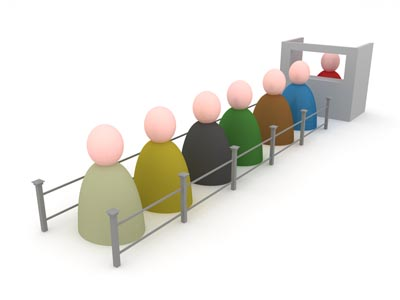
\includegraphics[width=7.553cm,height=4.357cm]{image/a2012Logique2eme-img013.jpg}
\end{center}
	

%===================
\section{Définition}
%===================
	
	\marginicon{file}	
	Une \textbf{file} est une collection d'éléments 
	admettant les fonctionnalités suivantes~:

	\begin{itemize}
		\item {
			on peut toujours ajouter un élément à la collection}
		\item {
			seul le premier élément ajouté peut être consulté ou enlevé}
		\item {
			on peut savoir si la collection est vide}
	\end{itemize}

	La file (en anglais \textit{queue}) est donc une collection 
	de données de type \textit{premier entré, premier sorti} 
	(en anglais on dit «~FIFO~», c'est-à-dire \textit{first in first out}). 
	L'analogie avec une file de clients à un guichet (poste, caisse du 
	supermarché {\dots}) est évidente~: c'est le premier arrivé qui est 
	le premier servi, et il est très malvenu d'essayer de doubler une personne 
	dans une file ! Noter qu'une fois entré dans une \textit{file} -- au
	sens informatique du terme -- on ne peut pas en sortir par l'arrière, 
	le seul scénario possible pour en sortir est
	d'attendre patiemment son tour et d'arriver en tête de la file.

	De même que pour la pile, on ne peut donc non plus parcourir une 
	file, ou consulter directement le \textit{n}\textsuperscript{ième}
	élément. Les files sont très utiles en informatique, citons par 
	exemple la création de mémoire tampon (\textit{buffer})
	dans de nombreuses applications, les processeurs multitâches 
	qui doivent accorder du temps-machine à chaque tâche, la
	file d'attente des impressions pour une imprimante {\dots}

%=====================================
\section{Implémentation orienté-objet}
%=====================================

	\subsection{Allure générale}
	%===========================
		
		Comme pour la pile, la classe File ne contient qu'un nombre 
		restreint de méthodes qui correspondent aux quelques
		opérations permises avec cette structure~: ajouter un élément 
		(\textit{«~enfiler~»}), consulter l'élément de tête, et
		le retirer (\textit{«~défiler~»}). Comme précédemment, nous ne 
		décrivons que les entêtes des constructeur et méthodes,
		le détail de l'implémentation sera laissé à titre d'exercices.

		\cadre{
			\begin{pseudo}
				\Class{File<T>}
				\RComment T est le type des éléments de la file
					\Private 
						\LComment {à détailler plus tard}
					\Public 
						\ConstrSign{File<T>}{}
						\RComment crée une file vide
						\MethodSign{enfiler}{élément~: T}{}
						\RComment ajoute un élément dans la file
						\MethodSign{tête}{}{T}
						\RComment retourne la valeur de l'élément en tête de file, sans le retirer
						\MethodSign{défiler}{}{T}
						\RComment enlève et retourne l'élément de tête
						\MethodSign{estVide}{}{booléen}
						\RComment indique si la file est vide
				\EndClass
			\end{pseudo}
		}
		
	\subsection{Remarques~:}
	%=======================
		
		\begin{itemize}
			\item 
				De même que dans le chapitre précédent, la file est supposée 
				\textit{infinie}, c'est-à-dire qu'on peut y ajouter un
				nombre indéterminé d'éléments. Le cas de la file limitée à 
				une capacité maximale sera envisagé dans l'exercice 2.
			\item
				Dans l'implémentation, il faudra songer à envoyer un message 
				d'erreur lorsqu'on utilise les méthodes \textit{tête} et
				\textit{défiler} si la file est vide. Si la file possède une 
				taille maximale, alors c'est \textit{enfiler} qui doit
				générer un message d'erreur lorsque la file est pleine.
		\end{itemize}

	
%==================
\section{Exercices}
%==================

	\begin{Exercice}{Implémentation via une liste chainée bidirectionnelle}
		
		Détaillez l'implémentation de la classe file en utilisant 
		comme représentation des données une liste chainée bidirectionnelle.
	\end{Exercice}

	\begin{Exercice}{La file de taille limitée}
		
		La file de taille limitée ne peut contenir au plus qu'un nombre d
		onné d'éléments. On demande d'implémenter ce type de
		file en utilisant un tableau. Les attributs privés de la 
		classe seront les suivants~:

		\cadre{
			\begin{pseudo}
				\Class{File<T>}
					\Private
						\Decl tab~: tableau de T 
						\RComment tableau (dynamique) contenant les éléments de la file
						\Decl premier~: entier
						\RComment indice du premier élément entré (tête de file)
						\Decl dernier~: entier
						\RComment indice du dernier élément entré (fin de file)
						\Decl tailleMax~: entier
						\RComment taille maximale de la file
					\EndClass
			\end{pseudo}
		}
				
		Nous proposons ici d'offrir un constructeur qui reçoit la 
		taille maximale de la file et qui crée un tableau d'indices 0
		à tailleMax (le tableau aura donc un élément de plus que 
		la taille maximale de la file, nous allons expliquer
		pourquoi). On remplit le tableau en ajoutant les éléments les 
		uns à la suite des autres en retenant la position du
		premier et du dernier via deux indices. Lorsqu'on ajoute un élément, 
		la position du dernier va augmenter, et lorsqu'on
		enlève un élément, cela revient à augmenter la position du premier, 
		afin d'éviter de devoir retasser l'ensemble de la
		file en début de tableau, ce qui serait une perte d'efficacité.

		\textbf{Exemple~:}

		Supposons qu'après la création de la file, les éléments 4, 3, 6 et 2 
		ont été ajoutés. L'indice du premier est 0 et celui du dernier est 3.

		\begin{center}
			\tablefirsthead{}
			\tablehead{}
			\tabletail{}
			\tablelasttail{}
			\begin{supertabular}{|m{1.171cm}|m{1.206cm}|m{1.206cm}|m{1.206cm}|m{1.206cm}|m{1.206cm}|m{1.206cm}|m{1.206cm}|m{1.206cm}|m{1.232cm}|}
			\hline
			\centering{\sffamily 4} &
			\centering{\sffamily 3} &
			\centering{\sffamily 6} &
			\centering{\sffamily 2} &
			~
			 &
			~
			 &
			~
			 &
			~
			 &
			~
			 &
			~
			\\\hline
			\end{supertabular}
		\end{center}
		
		On ajoute l'élément 7. L'indice du dernier est à présent 4.

		\begin{center}
			\tablefirsthead{}
			\tablehead{}
			\tabletail{}
			\tablelasttail{}
			\begin{supertabular}{|m{1.171cm}|m{1.206cm}|m{1.206cm}|m{1.206cm}|m{1.206cm}|m{1.206cm}|m{1.206cm}|m{1.206cm}|m{1.206cm}|m{1.232cm}|}
			\hline
			\centering{\sffamily 4} &
			\centering{\sffamily 3} &
			\centering{\sffamily 6} &
			\centering{\sffamily 2} &
			\centering{\sffamily 7} &
			~
			 &
			~
			 &
			~
			 &
			~
			 &
			~
			\\\hline
			\end{supertabular}
		\end{center}
		
		On enlève un élément de la file. L'indice du premier vaut maintenant 1

		\begin{center}
			\tablefirsthead{}
			\tablehead{}
			\tabletail{}
			\tablelasttail{}
			\begin{supertabular}{|m{1.171cm}|m{1.206cm}|m{1.206cm}|m{1.206cm}|m{1.206cm}|m{1.206cm}|m{1.206cm}|m{1.206cm}|m{1.206cm}|m{1.232cm}|}
			\hline
			~
			 &
			\centering{\sffamily 3} &
			\centering{\sffamily 6} &
			\centering{\sffamily 2} &
			\centering{\sffamily 7} &
			~
			 &
			~
			 &
			~
			 &
			~
			 &
			~
			\\\hline
			\end{supertabular}
		\end{center}
		
		Ce mécanisme peut se faire de façon circulaire~: arrivés en fin 
		de tableau, les indices premier et dernier repassent à
		0. Lorsque premier et dernier sont égaux, la file n'a qu'un 
		seul élément. Si cet élément est supprimé, l'incrémentation
		de premier aura pour conséquence que l'indice premier sera 
		d'une unité supérieur à l'indice dernier (en tenant compte
		de la rotation des valeurs), et ce sera donc la condition 
		correspondant à une file vide. Le tableau ne sera jamais
		rempli au maximum pour pouvoir distinguer le cas d'une file 
		vide et le cas d'une file pleine. Nous placerons donc dans
		le tableau au maximum tailleMax éléments (en laissant un 
		élément «~vide~» entre les indices dernier et premier).
	\end{Exercice}
	
	\begin{Exercice}{Le monte-charge}
		
		Un monte-charge de chantier assure le transport de personnes 
		et de matériel entre deux niveaux. Lorsque le monte-charge
		arrive à un étage, tous ses passagers en sortent. La charge
		maximale admise à la valeur MAX (donnée en paramètre).
		Étant donné les risques liés à l'utilisation du monte-charge 
		en surcharge, le poids de chacun des passagers et des
		charges qu'ils transportent (outils, brouette de sable {\dots}) 
		est vérifié avant l'entrée dans le monte-charge.

		Pour gérer l'embarquement dans le monte-charge, on souhaite 
		faire appel à un algorithme «~embarquement~» qui détermine
		combien de personnes qui se trouvent actuellement 
		en file devant le monte-charge peuvent y entrer.

		Cet algorithme respectera l'ordre d'arrivée des personnes 
		et mettra à jour la file des personnes en attente qu'il aura
		reçue en paramètre.

		\begin{enumerate}
			\item {
				Choisissez une représentation de données adaptée à la solution du problème et justifiez votre choix. }
			\item {
				Écrivez l'algorithme «~embarquement~»}
			\item {
				Écrivez l'algorithme «~arrivée~» qui ajoute à la file une personne d'un poids donné en paramètre.}
			\item {
				Quels cas doit-on envisager ?}
		\end{enumerate}

	\end{Exercice}

	\begin{Exercice}{À l'envers}
	
		Écrire un module recevant en paramètre une file d'entiers. 
		À l'issue de ce module, les valeurs de la file seront en
		ordre inverse et débarrassées des éléments pairs.

		\textbf{Exemple~:} Si le contenu de la file est le suivant~:

		{\centering
		1 $\rightarrow $ 0 $\rightarrow $ 4 
		$\rightarrow $ 25 $\rightarrow $ 20 
		$\rightarrow $ 11 $\rightarrow $ 3 $\rightarrow
		$ 7 $\rightarrow $ 8 $\rightarrow $ 73 
		$\rightarrow $ 2 $\rightarrow $ 4
		\par}

		son contenu sera après traitement~: 

		{\centering 
		73 $\rightarrow $ 7 $\rightarrow $ 3 $\rightarrow 
		$ 11 $\rightarrow $ 25 $\rightarrow $ 1
		\par}

\end{Exercice}
	
		